\documentclass[12pt, a4paper, twocolumn]{article}
\usepackage[utf8]{inputenc}
\usepackage[cm]{fullpage}
\usepackage{fancyhdr}
\usepackage{textcomp}
\usepackage{graphicx}
\usepackage{hyperref}

\begin{document}

\title{Trabalho Final da Disciplina "Organização e Arquitetura de Computadores": PACMAN}
\author{
Arthur Bizzi: 13/0102636 \\
Arthur da Silveira Couto: 16/0002575 \\
Caio Albuquerque Brandão: 16/0003636 \\
Cristiano Silva Júnior: 13/0070629 \\
Leonardo Maffei: 16/0033811 \\}
\date{5 de Julho de 2017}
\maketitle

\section{Resumo}
Foi projetada e implementada uma versão do jogo Pac Man Battle Royale inteiramente em Assembly MIPS em um processador pipeline implementado pela classe. A implementação inclui em seus gráficos e interfaces, além de menu, cenário e personagem funcionais, inimigos dotados de Inteligência Artificial, sons, multiplayer e jogabilidade por controladores infravermelho.

\section{Introdução}
 O jogo Pac-Man foi criado em 1980 por Toru Iwatani em parceria com a Namco. Extremamente simples e popular, o jogo consiste em controlar o personagem titular, Pac-man, a caricata bola amarela antropomorfisada, em uma arena-labirinto onde ele deve fugir de fantasmas enquanto coleta pontos e procura por power ups.

 \begin{figure}[h!]
    \centering
    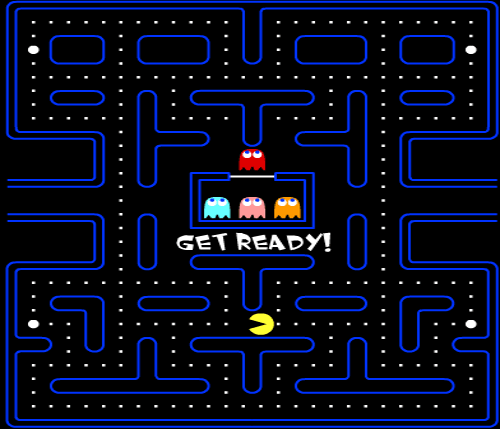
\includegraphics[width=0.4\textwidth]{pakku.png}
    \caption{O Pac-Man original}
\end{figure}

Pac Man Battle Royale é a mais recente iteração da clássica série de jogos. Essa versão, lançada pela Namco em 2011, foi criada para a nova geração de computadores e consoles e conta com dois principais diferenciais: Melhorias gráficas e um modo \textit{multiplayer} competitivo para até 4 jogadores. Essa é a versão do jogo que serviu como base e inspiração para nosso projeto, que busca ser uma reprodução tão fiel quanto possível do \textit{Battle Royale} numa plataforma Assembly MIPS.

O Assembly MIPS foi desenvolvido pela empresa MIPS Technologies, que buscava desenvolver um processador simples e barato para fins acadêmicos. Enquanto arquitetura, ela foi desenvolvida seguindo o padrão \textit{load-store}, também conhecido como \textit{registrador-registrador}, isto é, todas as operações recuperam e armazenam dados nos registradores somente. A exceção são as instruções de \textit{load} e \textit{store}, as únicas capazes de operar com a memória principal.

Para simular programas escritos para a arquitetura MIPS, utilizamos o simulador MARS, que permite escrever e simular a execução de programas da tal arquitetura, além de compilá-los para um formato executável. O simulador também vem com diversas facilidades, como, por exemplo, uma tela própria para simular interfaces gráficas ou contadores de instruções para identificar o \textit{workload} de algum programa dado.

Para implementar a organização do processador MIPS, utilizamos a linguagem \textit{Verilog}, utilizada para descrever hardware. O código é compilado para ser utilizado na FPGA \textit{Altera DE-II Cyclone}, que implementa o processador em um meio físico, permitindo que os executáveis possam interagir com o mundo real. No caso, essa interação é fundamental, pois o jogo em questão necessita de \textit{feedback} dos usuários por meio de controles remotos, como especificado.

O objetivo principal do processador é um implementar a organização \textit{pipeline}, que se baseia na execução em paralelo de microinstruções. Nela, o processador é dividido em alguns circuitos principais (denominados  estágios) que podem executar tarefas em separado e repassar seus resultados para o estágio seguinte. Desta forma, todas as instruções da arquitetura devem ser trabalhadas para que elas sejam executadas nas etapas determinadas para o \textit{pipeline}.

O pipeline clássico tem 5 estágios:

\begin{itemize}
    \item Leitura da instrução
    \item Decodificação da instrução
    \item Execução da instrução
    \item Operações com a memória principal
    \item Escrita nos registradores
\end{itemize}

Como as instruções são executadas em paralelo, podemos ter problemas do gênero \textit{race condition} entre as instruções, isto é, uma instrução depender do resultado de uma instrução que ainda não foi completa. Para tanto, podemos adaptar o programa para que isto não aconteça ou adaptar o \textit{hardware} para detectar quando que isso ocorre e colocar \textit{locks} (comumente chamadas de "bolhas") no pipeline, isto é, fazer com que as instruções que dependam de algum dado esperem pelo fim da execução da instrução.


\section{Metodologia}

O jogo foi inteiramente programado em assembly MIPS, sendo posteriormente otimizado para um processador \textit{pipeline} que rodaria na placa \textit{Altera DE-II Cyclone}.

A idea principal da implementação do jogo segue uma arquitetura de software \textit{Model-View-Controller}. Basicamente, temos um \textit{loop} principal que sempre checa por entradas e atualiza a tela do jogo. Novas entradas do usuário causam efeitos colaterais que levam o jogo a novos estados. No caso, temos 2 grandes estados principais: o menu principal, que serve para configurar o jogo; e o jogo em si, em que os jogadores podem andar pelo labirinto ao lado dos fantasmas controlados por uma inteligência artificial simples.

O processador implementado em Verilog é baseado em uma organização mínima desenvolvida em sala de aula pelo professor. Em cima dela, um processador mais completo, capaz de acessar dispositivos periféricos e operar com números em ponto flutuante, foi melhorado pelos alunos, tendo algumas modificações feitas pelo grupo para poder utilizar controles remotos e algumas operações com ponto flutuante a mais.

O processador segue uma organização em \textit{uniciclo}, onde todos os estágios executam de uma única vez por instrução a cada ciclo de clock.

\begin{figure*}[h!]
    \centering
    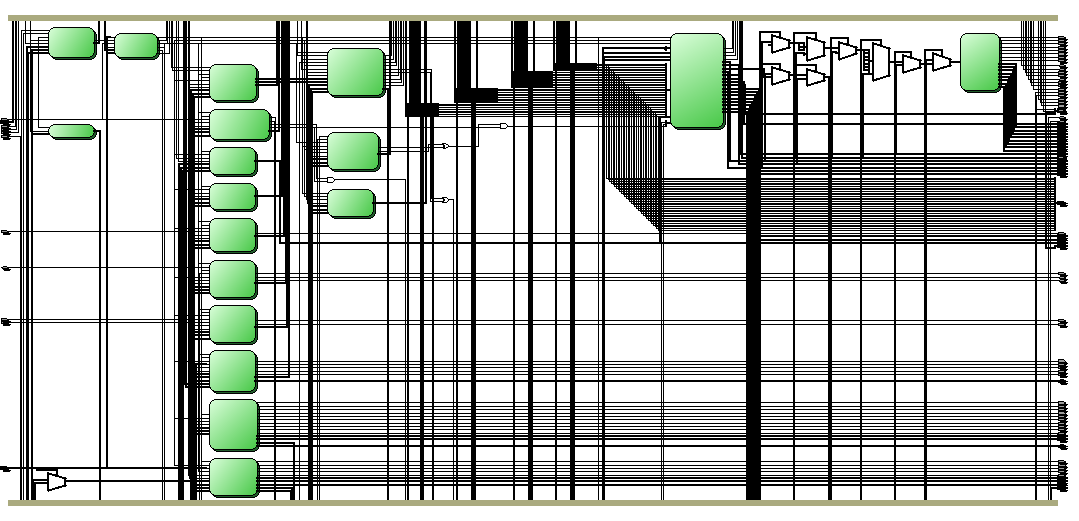
\includegraphics[width=0.8\textwidth]{data_unicicle.png}
    \caption{Ilustração do processador compilado em componentes lógicos}
\end{figure*}

\subsection{Apresentação e Menu}

A interface gráfica do jogo se dá por meio do carregamento de valores RGB da memória principal para um buffer do monitor, que sempre se atualiza mostrando, para cada pixel, um desses tais valores da memória. Para isso, temos um \textit{array} de endereços de memória reservados e mapeados para que o monitor possa ler em sequência e se atualizar.

O estilo gráfico simplificado do jogo se assemelha propositalmente a outros clássicos da era 8-16 bits, com contornos básicos e cores vibrantes. Os desenhos dos objetos mostrados em tela foram desenhados pixel a pixel e depois salvos na memória.

A primeira tela vista pelo jogador é o menu inicial. Nele, por meio de um dispositivo de entrada numérica, o usuário escolhe: o número de jogadores; o quantidade de vidas para cada um; e a quantidade de inimigos.

\begin{figure}[h!]
    \centering
    
\includegraphics[width=0.5\textwidth]{MENUPAC.jpeg}
    \caption{O menu simplificado: Número de jogadores}
\end{figure}

\newpage

 \begin{figure}[h!]
    \centering
    
\includegraphics[width=0.5\textwidth]{MENU.jpeg}
    \caption{Menu: Número de Fantasmas}
\end{figure}

\newpage

\subsection{Cenário e Movimentação}

Após a seleção dos parâmetros iniciais, o jogo é iniciado. O campo é uma \textit{maze} simétrica, na qual cada jogador começa em uma extremidade, que foi projetado de forma a se assemelhar às arenas do jogo original. Ele foi construído a partir da criação de um padrão \textit{ASCII} na região \textit{.data} da memória. Nesse carregamento, cada caractere corresponde a um tipo de célula no campo, e sua localização no vetor alocado determina sua posição no mapa.




O movimento se dá por entradas simples ($W$, $A$, $S$ e $D$) fornecidas pelos controladores de cada jogador. Essas entradas determinam a posição que o personagem tentará adentrar no próximo ciclo de jogo: $W$ o moveria para cima, $A$ para a esquerda, $S$ para baixo e $D$ para a direita. O movimento é bem sucedido se não houver colisão com um obstáculo, um fantasma ou outro jogador.

Obstáculos foram definidos na criação da arena e definem um espaço obstruído para transposição normal. Um movimento que adentraria território proibido é detectado e cancelado, mantendo o Pac-Man em seu caminho original.



\subsection{O Jogo: Pontuação e Vidas/\textit{Power-Ups}}
O objetivo do jogo é se deslocar pela arena, evitando os fantasmas quando se está vulnerável, destruindo-os quando se obtém o \textit{power up} e aumentando sua pontuação. No modo \textit{multiplayer}, entra o fator competitivo: Jogadores são encorajados a obter pontuações mais altas que seus adversários, para isso bloqueando suas trajetórias e destruindo-os por meio do uso do \textit{power up}.

Jogadores em movimento consomem esferas amarelas - denominadas \textit{comida} - que preenchem o estágio. Consumir essas esferas leva ao aumento de sua pontuação, visível no canto da tela ao lado do contador de corações. Ao final da partida, esse valor inteiro será o medidor de seu desempenho.

No decorrer da partida, os \textit{players} terão de admnistrar mais dois recursos: suas vidas e seus power-ups. As vidas (simbolizadas pelos corações na tela) determinam quantas chances ainda há de se voltar ao jogo após ser destruído por um inimigo. \textit{Power-ups}, por sua vez, \textit{power-up}, tornam o personagem capaz de destruir fantasmas e outros jogadores, e devem ser encontrados e coletados pela arena.

%TODO Adcionar um ultimo pedacinho de texto pra consertar a formatação dessa coluna

% TODO Colocar imagem do jogo com power-up

\subsection{Inimigos e AI}

Os fantasmas são os inimigos controlados pelo computador. Eles perseguem e cercam os jogadores, com o objetivo de os destruírem (removendo uma vida) caso os alcancem.

A movimentação dos fantasmas é determinada por uma inteligência artificial baseada no algoritmo de Dijkstra. O algoritmo de \textit{Pathfinding} é baseado no cálculo da menor distância a ser percorrida por cada fantasma para alcançar cada posição no mapa. Para cada fantasma, isso se dá pela geração recursiva de uma matriz que relaciona tiles no campo à quantidade de passos necessária para alcançá-los (associando  posições inacessíveis a $\infty$).

A trajetória do fantasma é então determinada localizando-se nessa estrutura o seu alvo - em geral o jogador mais próximo - e percorrendo-a retroativamente. Esse procedimento é reajustado a cada ciclo de jogo, de forma a se adaptar ao movimento de jogadores pela tela.

Esse procedimento é realizado de forma inteligente e unificada pelo conjunto de inimigos, o que possibilita movimentos coordenados em que um não atrapalha o outro, adaptando suas trajetórias para evitar olisões e Pac-Man perigosos (munidos de \textit{power up})

%Fantasmas evitam jogadores que pegaram o power up? O power Up está realmente implementado?


\subsection{Multiplayer e Controles Infravermelho}

Feito o jogo para um único jogador, implementar o modo multiplayer é apenas uma questão de expandir as possibilidades de entrada e modificar a inteligência artificial para se adaptar a perseguir vários jogadores, em geral optando por seguir o jogador mais próximo.

As diferentes formas de entrada, por sua vez, foram mapeadas a diferentes controladores infravermelho. Utilizando a convenção IrDA (Infrared Data Association), foi possível associar o sinal de cada controle disponível para a equipe a uma estrutura de entrada, que posteriormente é usada para controlar um personagem jogável.

\begin{figure*}[h!]
    \centering
    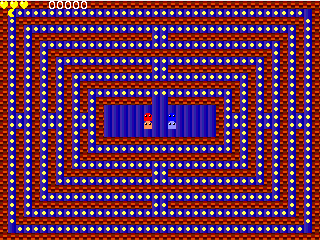
\includegraphics[width=0.65\textwidth]{JOGO1.png}
    \caption{O campo de jogo. Dimensões: 40x30}
\end{figure*}

%TODO: Foto dos controles infravermelhos? Seria Fera

\subsection{Som e Outros Detalhes de Software}

A implementação virtual do jogo conta com efeitos sonoros, que incluem um marcador de início de partida, sons de movimentação e um indicador de fim de jogo. Esses \textit{beeps} foram realizados pela chamada do procedimento \textit{syscall} com os argumentos adequados a cada turno de jogo.

\subsection{Implementação na Placa Cyclone DE II}

A equipe teve que analisar e criar código em linguagem de descrição de harware Verilog para tornar possível a execução do jogo no hardware da Altera. Isso incluiu, dentre outros, a implementação de novas instruções na unidade de ponto flutuante e adaptação de estruturas de entrada, saída e memória à realidade do hardware, utilizando seus mecanismos e switches com essa finalidade.

Foi também necessário realizar o ajuste de endereços de memória no código, de forma a controlar corretamente os dados na tela e na entrada. Além disso, a equipe teve que se adaptar à natureza distinta do processamento na placa, que frequentemente incorria em travamentos e comportamentos não previstos no processo de criação e simulação do software. Isso levou à análise do processamento código em configurações distintas de clock e ao acompanhamento passo a passo de instruções e seus efeitos na memória.

\section{Resultados Obtidos}

O resultado pode ser visto no YouTube no link \url{https://youtu.be/bpwdLiR33eU}.

A implementação na placa da Altera se mostrou um grande desafio. Estruturas funcionais da implementação do jogo no simulador MARS frequentemente não operavam como esperado ao passar o código pelo hardware da Cyclone II. Isso se dá, por exemplo, devido à ausência de alguma funções na ISA da placa, como mul e round, e complicações com hardware (buffers de teclado e procedimentos internos da placa). Além disso, posições de memória e parâmetros diversos diferiam nas duas aplicações.

Isso impediu o bom funcionamento da música e sons do jogo, por exemplo, e dificultou o processamento de entradas e saídas.

A execução do código em uma estrutura \textit{pipeline} real também apresentou desafios: A necessidade de inserção de bolhas nas instruções do código e a análise do código em Verilog para implementação em placa são exemplos disso.


\section{Conclusão}

A implementação complexa em Assembly do trabalho proposto demonstrou a possibilidade de utilizar a tecnologia diretamente em aplicações variadas, inclusive em algumas vistas classicamente como território da programação em alto nível, tais quais a criação de jogos, a implementação de inteligência artificial e o processamento de procedimentos recursivos.

O projeto também ocasionaou o melhor entendimento do processador estruturado em Pipeline. Seu caminho de dados, suas funções e seus hazards foram vistos na prática, permitindo o melhor entendimento de suas mecânicas. Isso inclui a percepção dos desafios que o Pipeline oferece: como custo de sua velocidade superior, ele apresenta maior complexidade e dificuldade de implementação. Essa percepção, acompanhada do fato de que essa arquitetura é amplamente majoritária em aplicações reais, é de grande importância.

O processador em \textit{pipeline} e o aprendizado dos conhecimentos requeridos para construí-lo e usá-lo são, de fato, a maior contribuição da disciplina.

\iffalse
\begin{figure}
    \centering
    \includegraphics[width=0.8\textwidth]{DIAG.jpg}
    \caption{Requisitos para FPULA sintetizada}
\end{figure}
\fi

\section{Referências Bibliográficas}

\begin{enumerate}
    \item PATTERSON, David A.. HENNESSY, John L. "Computer Organization and Design". 4th edition. Morgan-Kalman.
    \item MIPS32 Architecture For Programmers. MIPS Technologies.
    \item \url{http://pacman.com/en/pac-man-history}. Visitado em 4 de Julho de 2017.
    \item \url{https://courses.missouristate.edu/KenVollmar/mars/index.htm}. Visitado em 4 de Julho de 2017.
    \item \url{http://www.irda.org/}. Visitado em 4 de Julho de 2017.

\end{enumerate}

\end{document}
